\begin{center}
	\begin{circuitfig}[H]
		\centering
		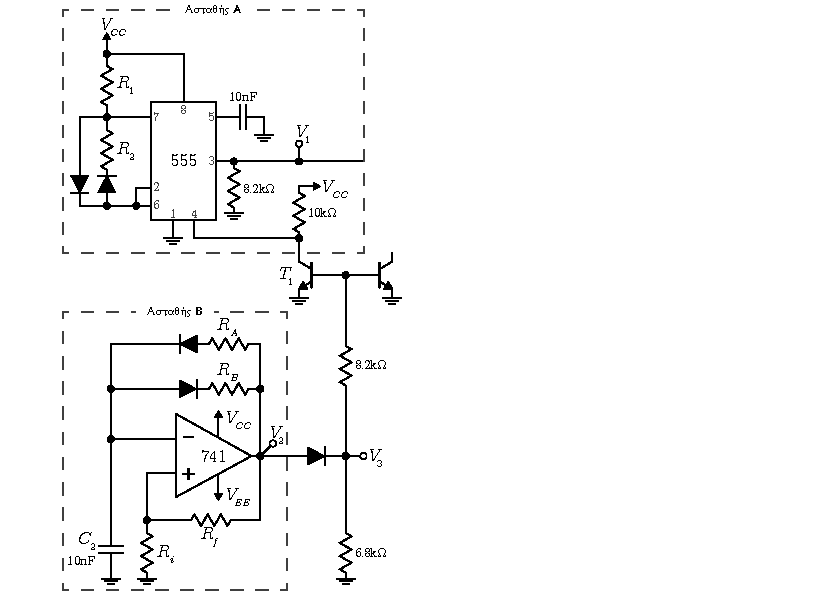
\includegraphics[width=14cm]{circuits/micro3_lab2.pdf}
		\caption{Γεννήτρια κλιμακωτής τάσης. Είναι $V_{CC}=15\unit{\volt}$ και $V_{EE}=-15\unit{\volt}$. Οι τιμές των αντιστάσεων που χρησιμοποιήθηκαν είναι $R_1=5.6\kohm$, $R_2=52\kohm$, $R_A=26\kohm$ και $R_B=180\kohm$.}
		\label{circ:2_schematic}
	\end{circuitfig}
\end{center}

\section{Θεωρητική μελέτη \& προσομοίωση}

	\subsection{Υπολογισμός στοιχείων του κυκλώματος}
		Απαιτείται, από την εκφώνηση, το ύψος κάθε βήματος να είναι $0.6\unit{\volt}$, η διάρκεια του κάθε βήματος $t_s=4\unit{\ms}$, η ολική διάρκεια της κλίμακας να είναι $t_o=20\unit{\ms}$ και τέλος η χρονική απόσταση μεταξύ των κλιμάκων να είναι $t_{\mathrm{H}}=3\unit{\ms}$. Παρακάτω παρατίθεται, εν συντομία, ο υπολογισμός των $t_{\mathrm{on}}$, $t_{\mathrm{off}}$, $R_1$, $R_2$, $R_A$ και $R_B$. Η λεπτομερής θεωρητική ανάλυση του κυκλώματος και η επεξήγηση της λειτουργίας του γίνεται στην επόμενη ενότητα.\par
Ξεκινώντας από τον ολοκληρωτή φαίνεται εύκολα πως
\begin{equation*}
	0.6\unit{\volt}=\frac{2}{RC}\int_{t_a}^{t_b}{V_1(t)\dd{t}},
\end{equation*}
όπου $t_a$ είναι μία χρονική στιγμή κατά την οποία η έξοδος του 555, $V_1$, περνάει από LOW σε HIGH και $t_b=t_a+t_{\mathrm{on}}$, όπου $t_{\mathrm{on}}$ η διάρκεια ενός διαστήματος στο οποίο η $V_1$ παραμένει σε HIGH. Με αριθμητική αντικατάσταση προκύπτει
\begin{equation*}
	0.6\unit{\volt}=\frac{2}{10\unit{\kilo\ohm}\cdot 1\unit{\micro\farad}}15\unit{\volt}\cdot t_{\mathrm{on}}\Rightarrow t_{\mathrm{on}}=400\unit{\micro\second}.
\end{equation*}

Εξαιτίας των διόδων στον ασταθή Α, ο πυκνωτής χωρητικότητας $C_1=0.1\unit{\micro\farad}$, του ασταθούς  Α, φορτίζεται προς $V_{CC}$ μόνο μέσω της $R_1$ και εκφορτίζεται προς τη γείωση μόνο μέσω της $R_2$. Επομένως είναι $t_{\mathrm{on}}=0.693\cdot C_1\cdot R_1$ και $t_{\mathrm{off}}=0.693\cdot C_1\cdot R_2$. Επιπλέον, η συνολική διάρκεια ενός βήματος είναι $t_s=t_{\mathrm{on}}+t_{\mathrm{off}}$. Με αριθμητική αντικατάσταση στην τελευταία σχέση προκύπτει $t_{\mathrm{off}}=3.6\unit{\ms}$.
\begin{equation*}
	R_1=\frac{t_{\mathrm{on}}}{0.693\cdot C_1}=\frac{0.4\unit{\ms}}{0.693\cdot 0.1\unit{\micro\farad}}\Rightarrow R_1=5.772\unit{\kilo\ohm}
\end{equation*}
και
\begin{equation*}
	R_2=\frac{t_{\mathrm{off}}}{0.693\cdot C_1}=\frac{3.6\unit{\ms}}{0.693\cdot 0.1\unit{\micro\farad}}\Rightarrow R_2=51.948\unit{\kilo\ohm}.
\end{equation*}

Περνώντας στον ασταθή πολυδονητή Β, ο πυκνωτής χωρητικότητας $C_2=0.1\unit{\micro\farad}$ φορτίζεται μέσω της $R_A$ και εκφορτίζεται προς τη γείωση μέσω της $R_B$. Συνεπώς, $t_o=t_{\mathrm{L}}=1.1R_B\cdot C_2$ και $t_{\mathrm{H}}=1.1R_A\cdot C_2$. Δηλαδή
\begin{equation*}
	R_Α=\frac{t_{\mathrm{H}}}{1.1\cdot C_2}=\frac{3\unit{\ms}}{1.1\cdot 0.1\unit{\micro\farad}}\Rightarrow R_A=27.272\unit{\kilo\ohm}
\end{equation*}
και
\begin{equation*}
	R_B=\frac{t_{\mathrm{L}}}{1.1\cdot C_2}=\frac{20\unit{\ms}}{1.1\cdot 0.1\unit{\micro\farad}}\Rightarrow R_B=181.818\unit{\kilo\ohm}.
\end{equation*}

	\subsection{Περιγραφή της λειτουργίας του κυκλώματος}
		\subsubsection{Ασταθής πολυδονητής Α}
	Το τερματικό 2 του 555 είναι το trigger $\mathrm{TR}$ και το τερματικό 6 είναι το threshold $\mathrm{TH}$. Όταν το 555 λαμβάνει ενεργό σήμα $\overline{\mathrm{TR}}$ η έξοδος του περνάει στο HIGH, κοντά στην τάση τροφοδοσίας $V_{CC}$ και παραμένει εκεί για χρόνο $t_{on}$ έως ότου να παρουσιαστεί ενεργό σήμα $\mathrm{TH}$. Τότε, η έξοδος του 555 περνάει στο LOW, κοντά στη γείωση.\cite{artofelectronics}\par
	Το $\overline{\mathrm{TR}}$ ενεργοποιείται από τάση μικρότερη του $\frac{1}{3}V_{CC}$, ενώ το $\mathrm{TH}$ από τάση μεγαλύτερη των $\frac{2}{3}V_{CC}$.\cite{artofelectronics}\cite{sedra}\cite{scherz}\par
	Ο πυκνωτής $C_1$ αρχίζει να φορτίζεται προς $V_{CC}$ μόλις το κύκλωμα συνδεθεί στην τροφοδοσία.\cite{scherz} Η φόρτισή του, λόγω των δύο διόδων, γίνεται μόνο μέσω του ωμικού αντιστάτη $R_1$. Η έξοδος του χρονιστή 555 βρίσκεται σε στάθμη HIGH όσο ο πυκνωτής φορτίζεται. Μόλις ο πυκνωτής $C_1$ ξεπεράσει τα $\frac{2}{3}V_{CC}$ το σήμα $\mathrm{TH}$ γίνεται ενεργό και το $\overline{\mathrm{TR}}$ απενεργοποιείται, οδηγώντας την έξοδο σε στάθμη LOW για χρονικό διάστημα $t_{off}$, και ο πυκνωτής αρχίζει να εκφορτίζεται, μέσω του $R_2$, προς τη γείωση.\cite{artofelectronics}\par
	Βάσει των παραπάνω, η τάση του πυκνωτή $C_1$ είναι $\frac{1}{3}V_{CC}\leqslant V_{C1}\leqslant\frac{2}{3}V_{CC}$ και η περίοδος του παλμού\footnote{Εάν δεν υπήρχαν οι δίοδοι θα ήταν $T=0.693\cdot\(R_1+2R_2\)$.\cite{artofelectronics}\cite{sedra}\cite{scherz}} είναι $T=t_s=0.693\cdot(R_1+R_2)\cdot C_1$. Εφόσον είναι $T=t_s=t_{on}+t_{off}$ και οι δίοδοι ορίζουν δύο ξεχωριστές διαδρομές για τη φόρτιση και την εκφόρτιση του πυκνωτή, θα είναι $t_{on}=0.693\cdot R_1\cdot C_1$ και $t_{off}=0.693\cdot R_2\cdot C_1$. Τέλος, ο κύκλος εργασίας (duty cycle), $\sfrac{t_{on}}{t_s}$, είναι προφανές πως ισούται με $\sfrac{R_1}{\(R_1+R_2\)}$.\par
	% TODO:
	% + διάγραμμα V1

\subsubsection{Ασταθής πολυδονητής Β}

	\subsection{Temperature sweep}
		Έγινε προσομοίωση του κυκλώματος στις θερμοκρασίες $-20\unit{\celsius}$, $0\unit{\celsius}$, $20\unit{\celsius}$, $35\unit{\celsius}$ και $70\unit{\celsius}$ και παρατηρήθηκε η κυματομορφή της εξόδου. Τα αποτελέσματα φαίνονται στο διάγραμμα \ref{plot:2_temp}.\par

\begin{table}[h]
	\begin{center}
		\begin{tabular}{|l |c |c |c |c |c |}
			\specialrule{1.25pt}{0pt}{0pt}
			\textbf{PSpice measurement} & $-20\unit{\celsius}$           & $0\unit{\celsius}$             & $20\unit{\celsius}$            & $35\unit{\celsius}$            & $70\unit{\celsius}$            \\\hline\hline
			\texttt{Max(V(U2:OUT))}     & $6.79172\unit{\volt}$          & $6.76318\unit{\volt}$          & $6.72997\unit{\volt}$          & $6.68878\unit{\volt}$          & $6.63272\unit{\volt}$          \\\hline
			\texttt{Period(V(U2:OUT))}  & $23.84931\unit{\milli\second}$ & $23.75302\unit{\milli\second}$ & $23.65926\unit{\milli\second}$ & $23.58503\unit{\milli\second}$ & $23.37579\unit{\milli\second}$ \\\specialrule{1.25pt}{0pt}{0pt}
		\end{tabular}
		\caption{Μετρήσεις των κυματομορφών του διαγράμματος \ref{plot:2_temp}.}
		\label{table:ask2:q5}
	\end{center}
\end{table}

Από τον πίνακα \ref{table:ask2:q5} προκύπτει πως η αύξηση της θερμοκρασίας μειώνει την μέγιστη τάση της κλίμακας αλλά μειώνει και την περίοδό της. Από το διάγραμμα \ref{plot:2_temp} φαίνεται πως η αύξηση της θερμοκρασίας μετατοπίζει την κυματομορφή ελαφρώς προς τα αριστερά.\par

\begin{plot_fig}
	\centering
	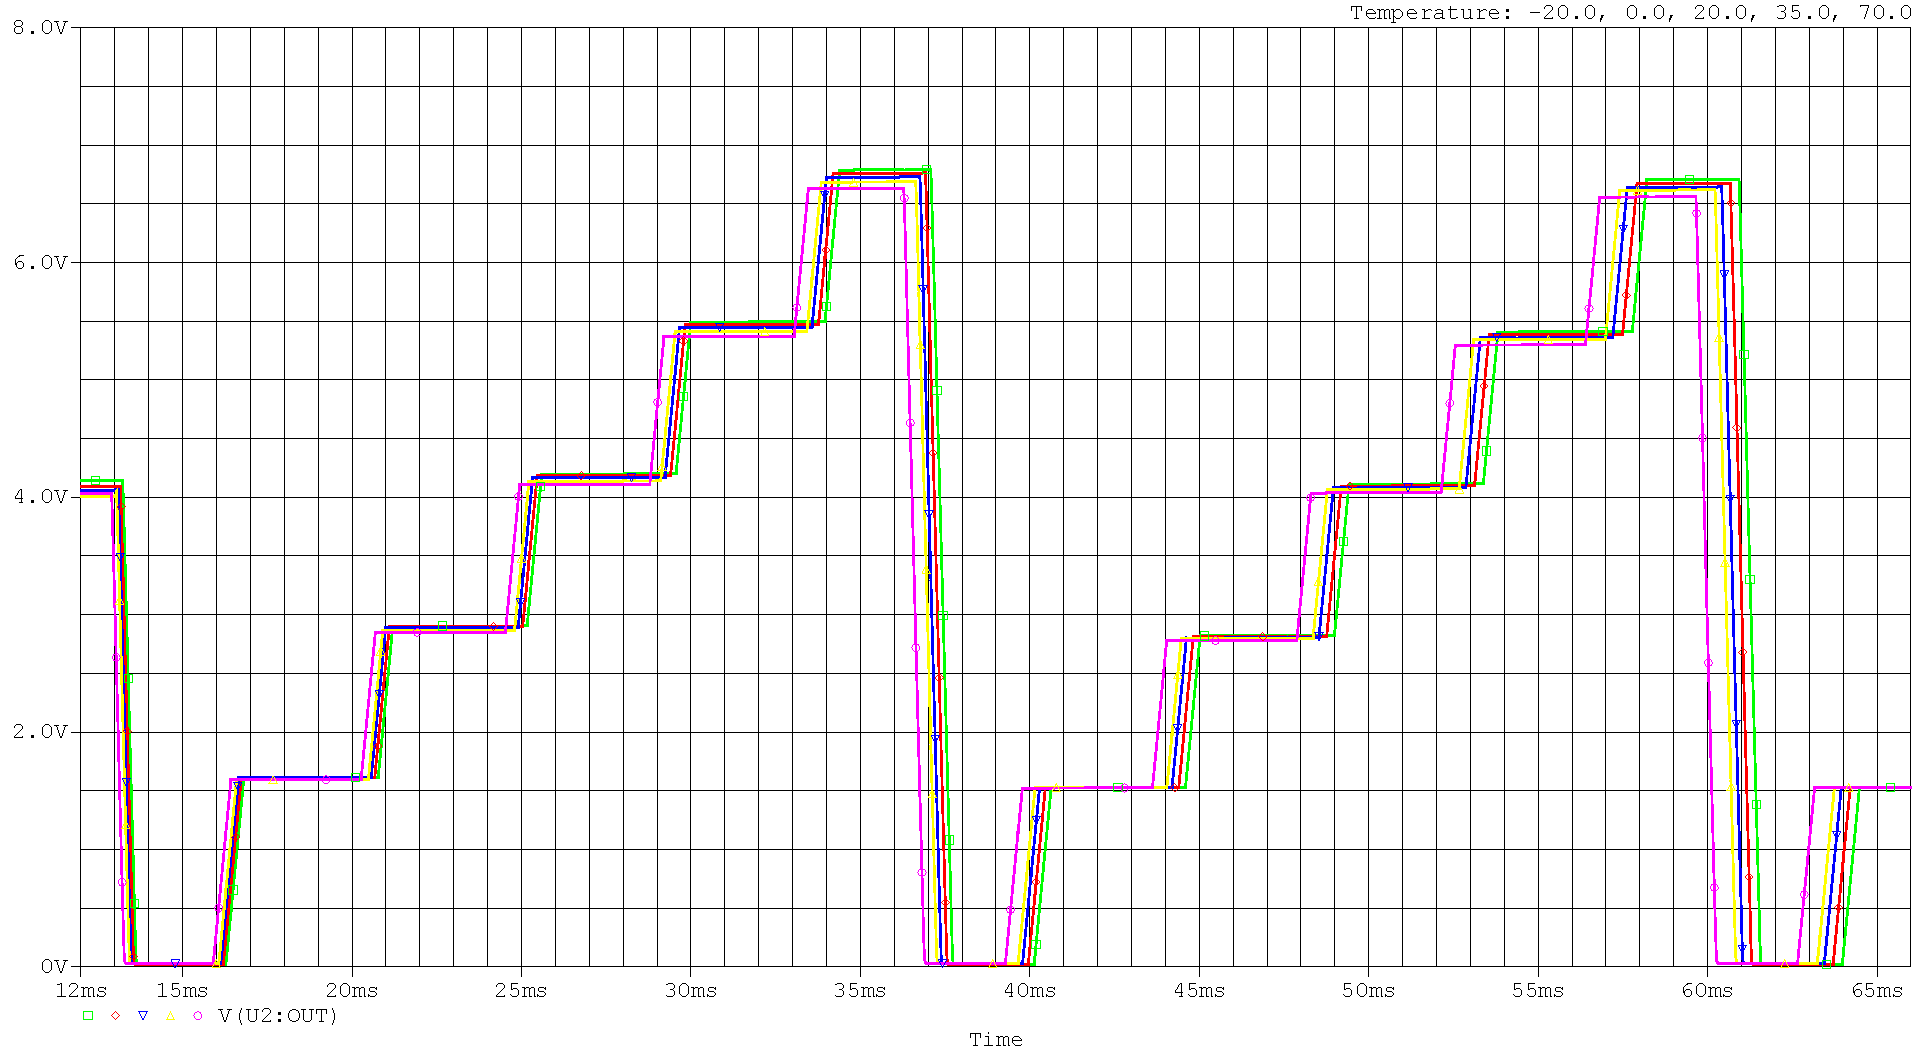
\includegraphics[width=13cm]{spice_02/q5.pdf}
	\label{plot:2_temp}
	\caption{Temperature sweep. Οι κυματομορφές στο υπόμνημα, από αριστερά προς δεξιά, αντιστοιχούν στις θερμοκρασίες $-20\unit{\celsius}$, $0\unit{\celsius}$, $20\unit{\celsius}$, $35\unit{\celsius}$ και $70\unit{\celsius}$.}
\end{plot_fig}
\vspace*{0.25cm}

	\subsection{Χαρακτηριστικές $v_{CE}-i_C$ BJT}
		\begin{center}
	\begin{circuitfig}[H]
		\centering
		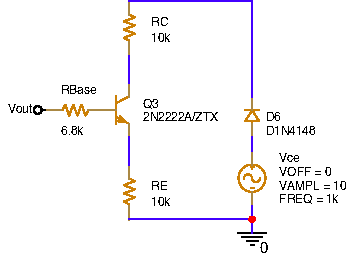
\includegraphics[width=6cm]{spice_02/ask2_bjt_schematic.pdf}
		\caption{Κύκλωμα για τη λήψη των χαρακτηριστικών $v_{CE}-i_C$ ενός BJT. Το κύκλωμα συνδέεται στην έξοδο της γεννήτριας κλιμακωτής τάσης.}
		\label{circ:2_bjt_schematic}
	\end{circuitfig}
\end{center}

Η μεταβολή του ρεύματος στη βάση του transistor επιτυγχάνεται μέσω της μεταβολής της τάσης στην έξοδο της γεννήτριας. Η εναλλασσόμενη πηγή τάσης \texttt{Vce} έχει περίοδο $T_{v_{CE}}=\sfrac{1}{1\unit{\kilo\hertz}}=1\unit{\milli\second}$ αρκετά μικρότερη από την διάρκεια κάθε βήματος της γεννήτριας, $t_s=$. Επομένως, το ρεύμα στη βάση του transistor παραμένει σταθερό για αρκετό χρόνο ώστε να ολοκληρωθεί η σάρωση της διαφοράς δυναμικού μεταξύ συλλέκτη και εκπομπού.\par
Η προσομοίωση γίνεται στο πεδίο του χρόνου σε διάστημα μίας περιόδου της κλιμακωτής τάσης. Μέσω των ρυθμίσεων των αξόνων στο PSpice, επιλέγεται η διαφορά δυναμικού μεταξύ συλλέκτη και εκπομπού ως η μεταβλητή του οριζόντιου άξονα. Ως \texttt{trace} του γραφήματος επιλέγεται το ρεύμα στον εκπομπό. Τα αποτελέσματα της προσομοίωσης φαίνονται στο διάγραμμα \ref{plot:2_bjt}.\par

\begin{plot_fig}[H]
	\begin{center}
		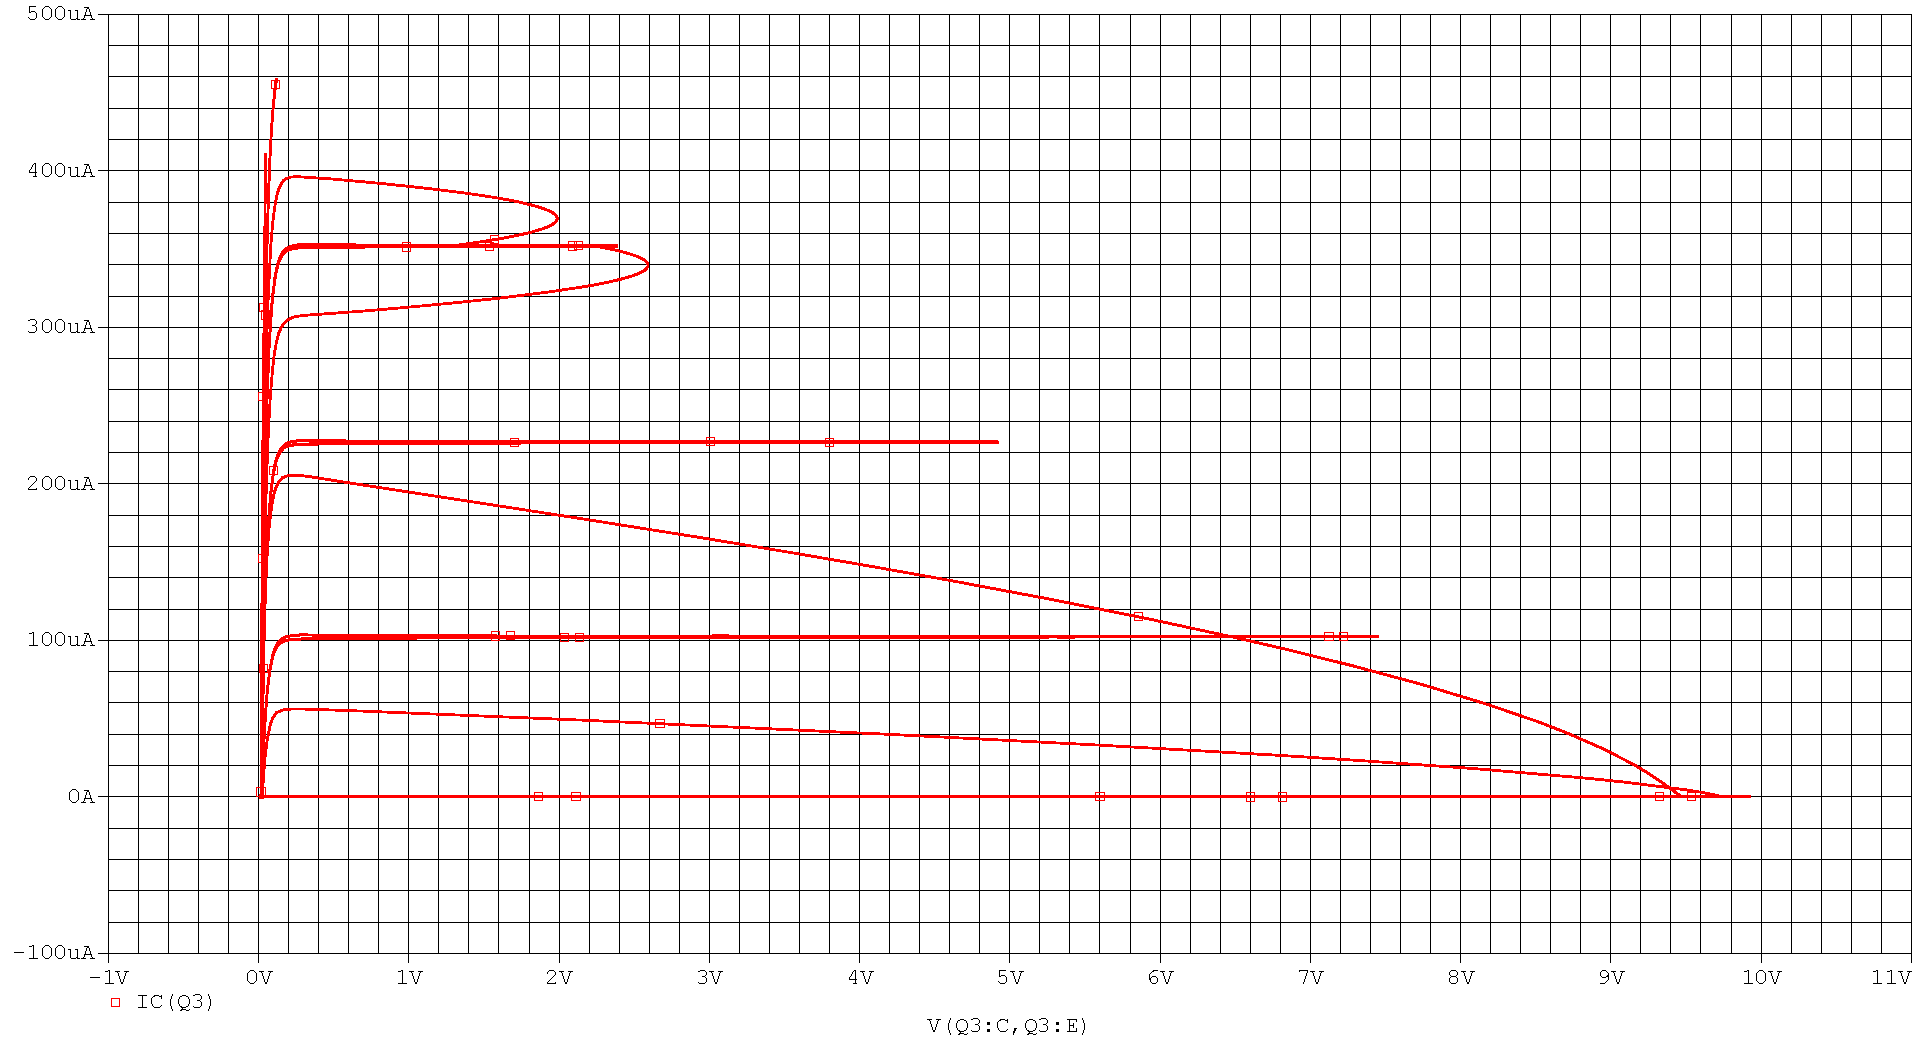
\includegraphics[width=\linewidth]{spice_02/q6.pdf}
		\caption{Χαρακτηριστικές $v_{CE}-i_C$. Οι \textsl{ενδιάμεσες} καμπύλες, μεταξύ των αναμενόμενων καμπυλών, οφείλονται στο γεγονός πως καθώς μεταβάλλεται η έξοδος της γεννήτριας η σάρωση της πηγής \texttt{Vce} του κυκλώματος \ref{circ:2_bjt_schematic} συνεχίζεται.}
		\label{plot:2_bjt}
	\end{center}
\end{plot_fig}

\newpage
\section{Εργαστηριακή εφαρμογή}
	\subsection{Λήψη κυματομορφών $v_1$, $v_{C_1}$ και $v_2$}
Οι κυματομορφές $v_1$, $v_{C_1}$ και $v_2$ του κυκλώματος \ref{circ:2_schematic}  δίδονται στο διάγραμμα \ref{plot:2.2_lab_voltages}.

\begin{chart}[H]
	\begin{center}
		\pgfplotsset{grid style={dotted,lightgray}}
\begin{tikzpicture}
	\begin{axis}[
			scale only axis,
			height=4cm,
			width=5cm,
			grid=both,
			minor tick num=1,
			xtick={0,1,2,3,4,5,6,7,8,9,10,11,12,13,14},
			ytick={-1.8,0,5,10,13},
			xlabel={Time $\(\unit{\milli\second}\)$},
			ylabel={Voltage $\(\unit{\volt}\)$}]

		\addplot+[thick,mark=none,const plot,color=DodgerBlue3]
		coordinates	{(1.5+0,-1.8) (1.5+0,13) (1.5+0.450,13) (1.5+0.450,-1.8) (1.5+4.500,-1.8)
				(1.5+4.500,13) (1.5+4.950,13) (1.5+4.950,-1.8) (1.5+9.000,-1.8)};
		\legend{$v_1$}
	\end{axis}
\end{tikzpicture}\hspace*{1cm}
\begin{tikzpicture}
	\begin{axis}[
			scale only axis,
			height=4cm,
			width=5cm,
			grid=both,
			minor tick num=1,
			ymin=-2.4,
			ymax=3,
			samples=200,
			ytick={-2.32,-2,-1,0,1,2,2.88},
			xlabel={Time $\(\unit{\milli\second}\)$},
			ylabel={Voltage $\(\unit{\volt}\)$}]

		\addplot[thick,color=DeepPink3,domain=-0.2:0.2] {1.225+3.1*(1-exp(-x*3.81))};
		\addplot[thick,color=DeepPink3,domain=0.2:4.14] {-4.76+8.11*exp(-x*0.29)};
		\addplot[thick,color=DeepPink3,domain=-0.2+4.34:4.34+0.2] {1.225+3.1*(1-exp(-(x-4.34)*3.81))};
		\addplot[thick,color=DeepPink3,domain=0.2+4.34:4.14+4.34] {-4.76+8.11*exp(-(x-4.34)*0.29)};
		\legend{$v_{C_1}$}
	\end{axis}
\end{tikzpicture}\vspace*{0.5cm}
\begin{tikzpicture}
	\begin{axis}[
			scale only axis,
			height=4cm,
			width=8cm,
			grid=both,
			minor tick num=3,
			ymin=-5,
			ymax=25,
			ytick={-4,0,10,20,24},
			xlabel={Time $\(\unit{\milli\second}\)$},
			ylabel={Voltage $\(\unit{\volt}\)$}]

		\addplot+[thick,mark=none,const plot,color=SeaGreen4]
		coordinates	{(0,-4) (0,24) (3,24) (3,-4) (23.4,-4)
				(0+23.4,-4) (0+23.4,24) (3+23.4,24) (3+23.4,-4) (23.4*2,-4)};
		\legend{$v_2$}
	\end{axis}
\end{tikzpicture}
		\caption{Οι τάσεις $v_1$, $v_{C_1}$ και $v_2$ όπως μετρήθηκαν χρήσει του παλμογράφου στο εργαστήριο.}
		\label{plot:2.2_lab_voltages}
	\end{center}
\end{chart}

Εφόσον η τροφοδοσία των τελεστικών ενισχυτών είναι $V_{CC}=15\unit{\volt}$ και $V_{EE}=-15\unit{\volt}$ είναι προφανές πως υπάρχει κάποιο offset στην τάση $v_2$ που παρατηρήθηκε στον παλμογράφο. καθώς η μέγιστη τιμή είναι $\max\(v_2\)=24\unit{\volt}>15\unit{\volt}$. Η σωστή κυματομορφή $v_2$ φαίνεται στο διάγραμμα \ref{plot:2.2b_lab_voltages}.\par
\begin{chart}[H]
	\begin{center}
		\pgfplotsset{grid style={dotted,lightgray}}
\begin{tikzpicture}
	\begin{axis}[
			scale only axis,
			height=5cm,
			width=10cm,
			grid=both,
			minor tick num=3,
			ymin=-14,
			ymax=15.5,
			ytick={-12.8,-10,0,10,14.4},
			xlabel={Time $\(\unit{\milli\second}\)$},
			ylabel={Voltage $\(\unit{\volt}\)$}]

		\addplot+[thick,mark=none,const plot,color=SeaGreen4]
		coordinates	{(0,-12.8) (0,14.4) (3,14.4) (3,-12.8) (23.4,-12.8)
				(0+23.4,-12.8) (0+23.4,14.4) (3+23.4,14.4) (3+23.4,-12.8) (23.4*2,-12.8)};
		\legend{$V_2$}
	\end{axis}
\end{tikzpicture}
		\caption{Η σωστή τάση $v_2$.}
		\label{plot:2.2b_lab_voltages}
	\end{center}
\end{chart}